% Chapter Template

\chapter{Introduction} % Main chapter title

\label{Chapter1} % Change X to a consecutive number; for referencing this chapter elsewhere, use \ref{ChapterX}

%----------------------------------------------------------------------------------------
%	SECTION 1
%----------------------------------------------------------------------------------------
%
% Statment of the problem + Motivation
%
Quantum computing is a new paradigm of computation whose importance is growing not only because of its promising speed-up over classical computers in some problems, such as combinatorial optimization problems, but also due to the fact that we are building transistors in a scale where quantum effects are starting to become relevant. Combinatorial optimization problems are common among industry albeit more research needs to be done to get insight about how quantum computing could help to solve industry challenges. There is already a large industry research in finance\,\cite{Herman2022AFinance}, route planning\,\cite{Tambunan2022QuantumSegment} and life sciences, among others. The research on applications of quantum computing to the energy sector has just began in the last years. There are only a few active research projects, like Q-Grid by e-On\,\cite{Fernandez-Campoamor2021CommunityAnnealing} or EnerQuant by Fraunhofer. The goal of this work to contribute to this field of research.
\begin{figure}[H]
  \begin{center}
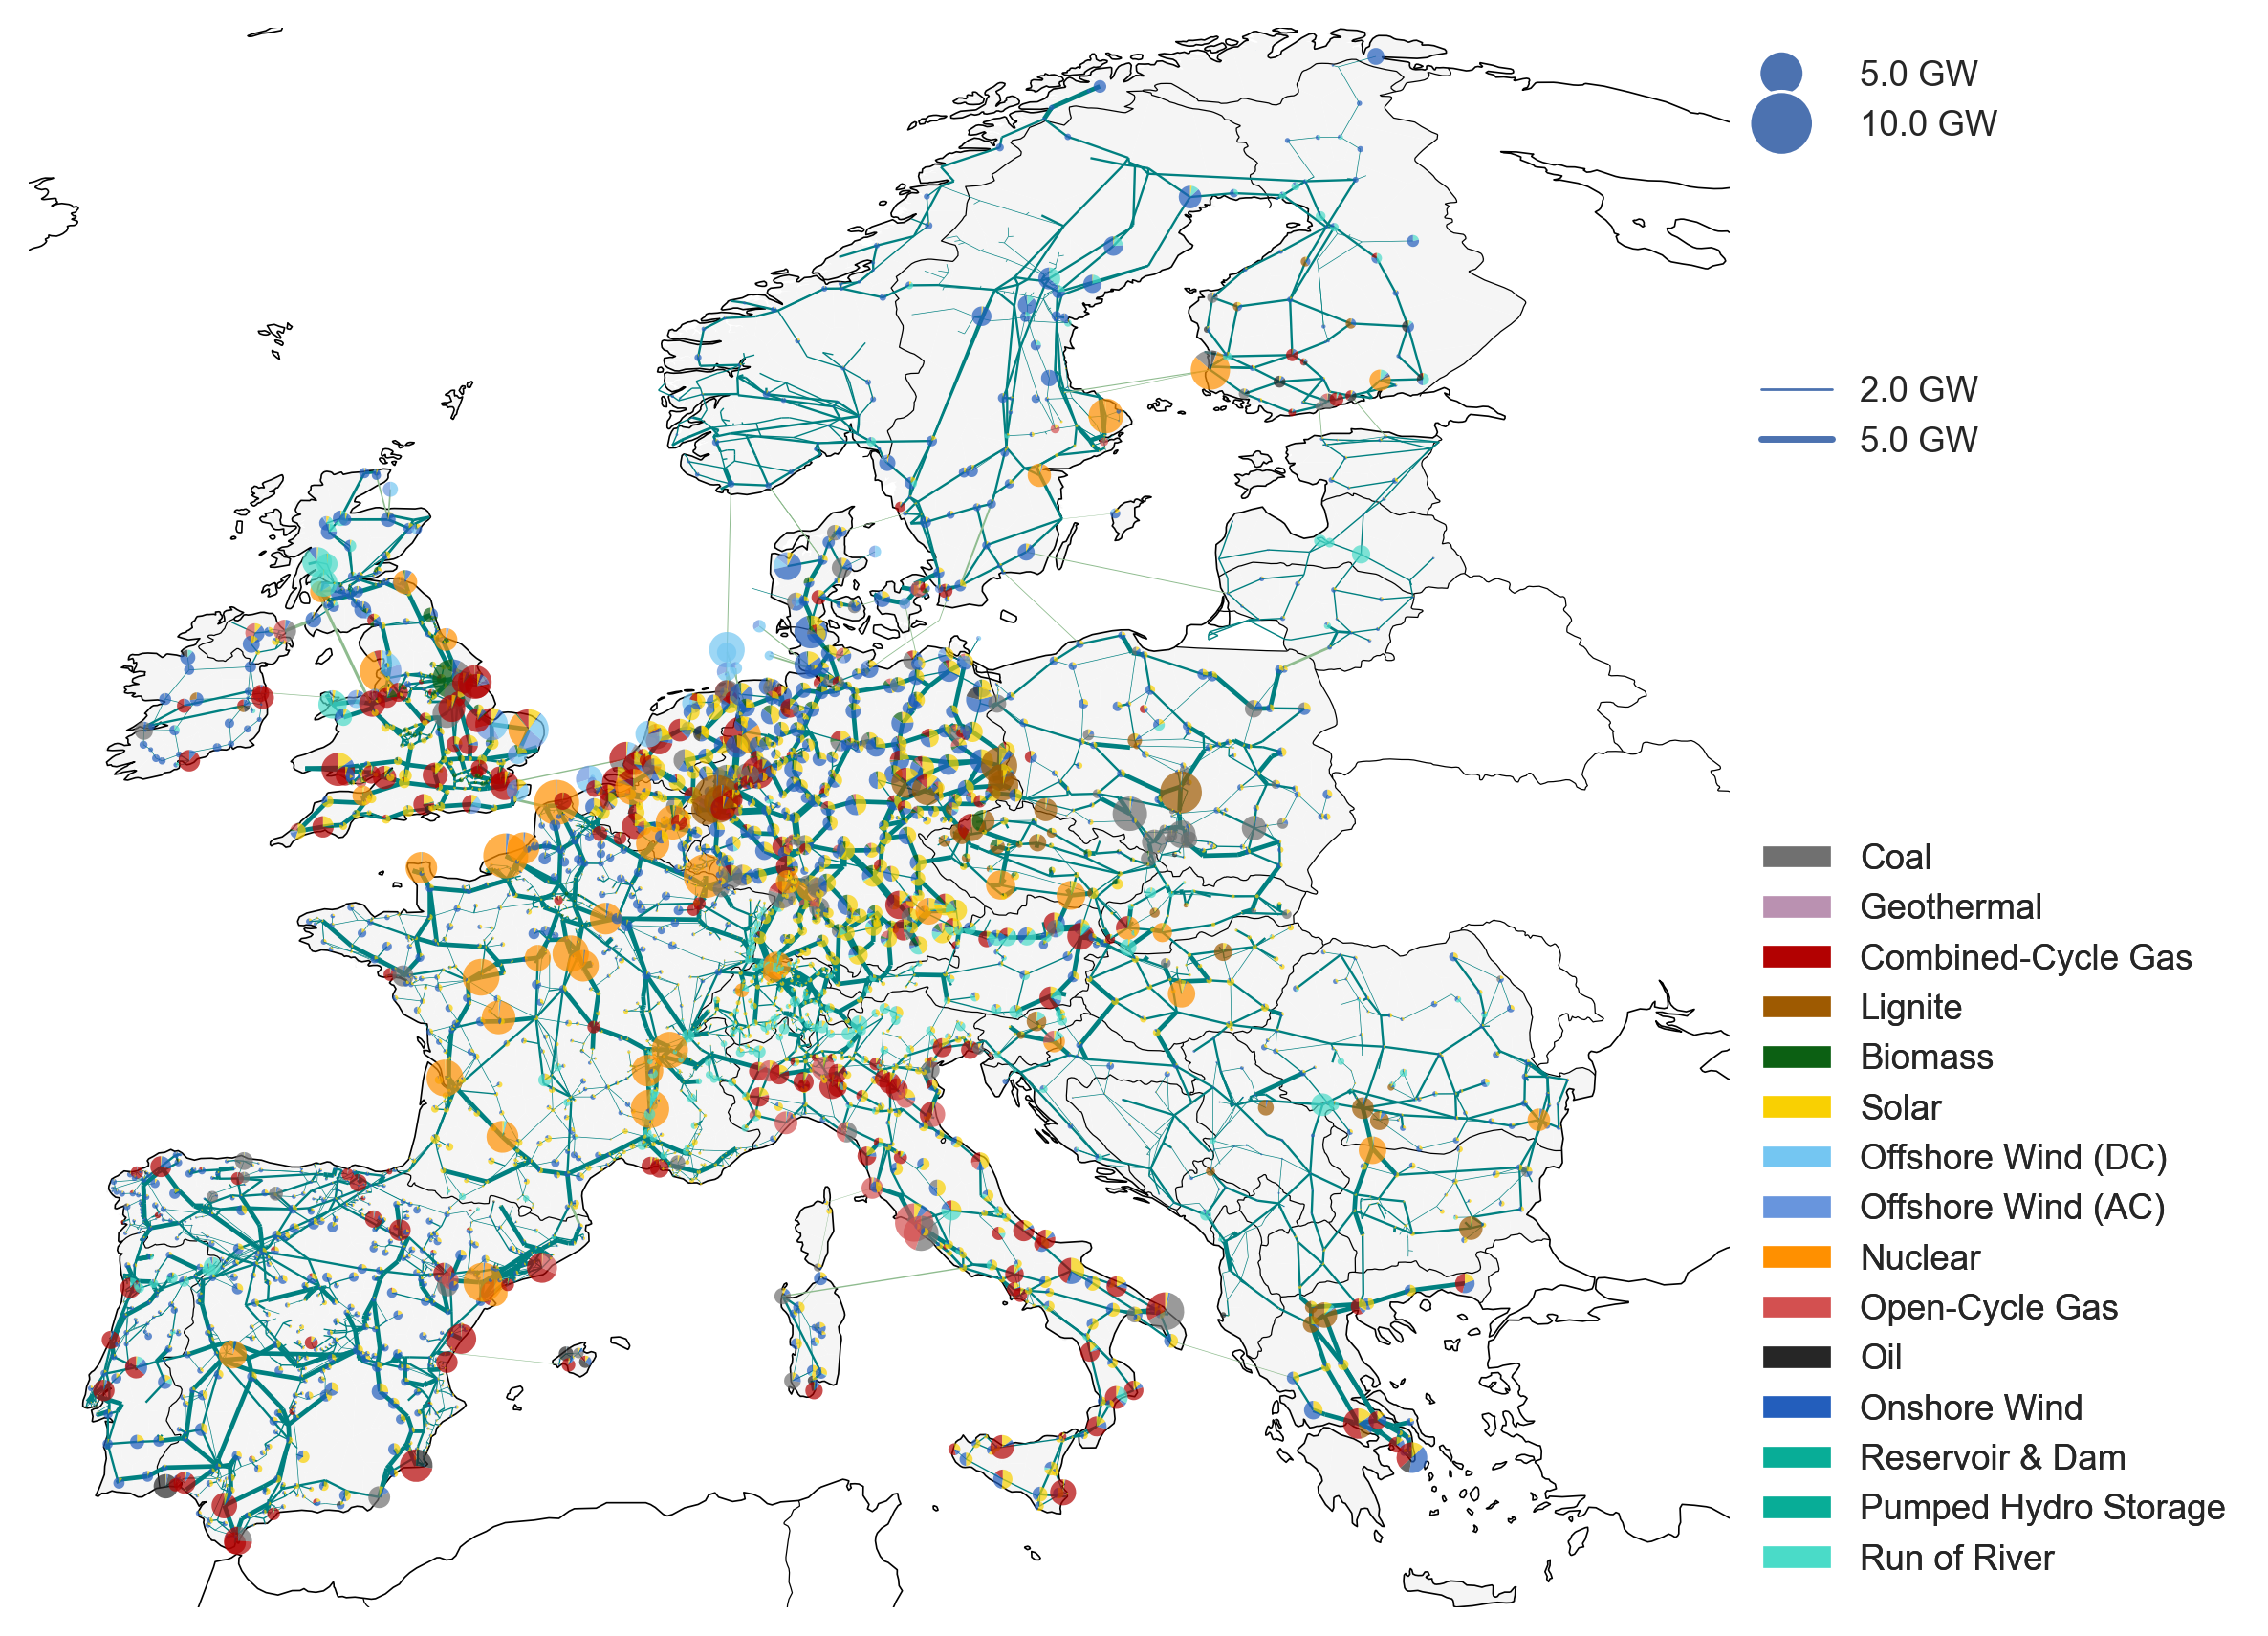
\includegraphics[width=0.85\textwidth]{Figures/Europe-Grid.png}
  \end{center}
  \caption{Clustered European transmission network model obtained from PyPSA-EUR\,\cite{PyPSA-Eur:PyPSA-Eur}.}
\end{figure}
Energy system models are getting larger and more complex due to the integration of decentralized weather-dependent renewable energy sources, intermittent loads, sector coupling and the increase of storage components. For instance, the renewable energy produced by the integration of solar panels in dwellings is intended to be integrated to the grid if consumers are not using it. However, the grid infrastructure is not evolving accordingly to the new energy paradigm. As a consequence, energy from private sources cannot be added to the grid, which implies the efficiency of solar panels has to be decreased or the excess of energy has to be discarded. An accurate expansion planning would solve these problems by redirecting the excess of energy to where it is required or by storing it so that it can be used later, e.g., to charge an electric car. In this way, the energy would be efficiently distributed and energy companies could offer better prices to their consumers while safeguarding the environment by reducing their carbon footprints. Furthermore, an increment of the quantity of detailed data about energy consumption -- smart meters -- would extend the spatial and temporal resolution, i.e., the grid status of a region, so that better managing and expansion planning decisions can be made in order to satisfy the customer demand efficiently.\\\\ 
The problem we tackle in the present work is called \textit{transmission expansion planning} (TEP) problem, which is a \textit{mixed-integer linear programming} (MILP) problem with NP complexity, that aims at finding the optimal way to expand the capacity and connections of an energy system. Currently, the scope and granularity of the model are reduced using clustering algorithms. For this reason, any computational time reduction will have substantial implications in closing the granularity gap between what the current models can solve and the desired resolution needed by energy system operators.\\\\
Quantum computers are the candidates to solve NP-hard problems such as MILP, by making the complexity of the problem scale polynomically as the systems size grows. Concretely, quantum analog computers are special-purpose quantum computers specialised in solving combinatorial optimization problems. The size of quantum analog computers that is the number of qubits of the system is greater than the general purpose quantum computers such as the ones from IBM that are based in the successive applications of quantum gates, such as the recently released Osprey quantum processor with 433 qubits.
%
% Objectives of my thesis
%
Although quantum computers are improving every few years they are not mature enough for solving many real-world problems where the number of variables scales exponentially. Also, we have to take into account that quantum computers are hugely affected by the environmental conditions\footnote{John Preskill called the current state of quantum technology as the Noisy Intermediate-Scale Quantum era, or NISQ for short\,\cite{Preskill2018}.} -- Noisy Intermediate-Scale Quantum (NISQ) era --, meaning that there will be errors during an algorithm execution, which implies that the execution time has to be short enough so that it does not exceed quantum decoherence. Because of the current maturity of quantum computers, hybrid quantum-classical approaches are required to tackle real-world problems\,\cite{Callison2022HybridBeyond}. The hybrid approach combines classical solvers and cutting-edge classical algorithms with quantum solvers that add the speed-up where it is possible.\\\\
A benchmark of how a TEP problem can be scaled up until current quantum solvers are not able to find a solution is provided among with a scheme to decompose a large TEP problem into a small enough master problem that can be addressed by a quantum computer and a sub-problem addressed by a classical computer. \\\\
% Structure of the thesis
%
The present work is structured as follows. Chapter\,\ref{Chapter2} guides through the foundations of adiabatic quantum computing. Chapter\,\ref{Chapter3} describes Benders' decomposition techniques in the field of quantum computing. Chapter\,\ref{Chapter4} solves a transmission expansion problem by starting with a small network solved by a pure quantum annealer and ending up with a bigger network that requires from hybrid solvers. Conclusions and outlook are drawn in Chapter\,\ref{Chapter5}.
